En este pasaje se muestran los diagramas de estados del sistema. Es así que se puede notar que el conjunto cuenta con 4 estados distintivos, siendo estos los llamados \textit{Initial}, \textit{Idle}, \textit{Charging} y \textit{Communicating}.

Vale la pena mencionar que en cualquiera de los estados, a excepción de \textit{Initial}, el sistema esta realizando mediciones del ambiente mientras cuenta también con la posibilidad de comunicarse por Bluetooth con la electrónica de la mochila. Esto se cumple excluyendo el caso en que el nivel de carga de la UBM no sea suficiente.

\begin{figure}[H]
	\centering
	%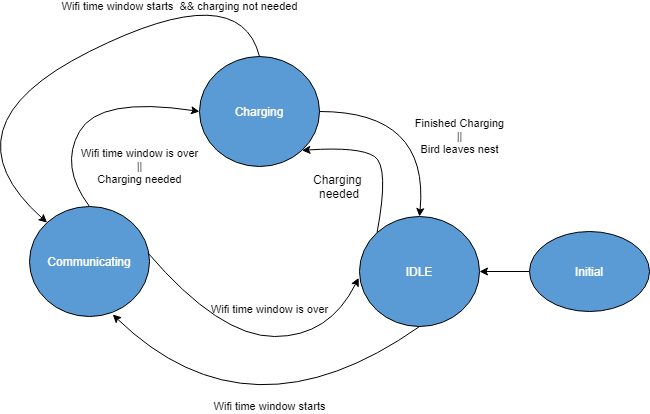
\includegraphics[width=0.9\linewidth]{ImagenesIngenieria de Detalle/Diagrama_de_Estados}	
	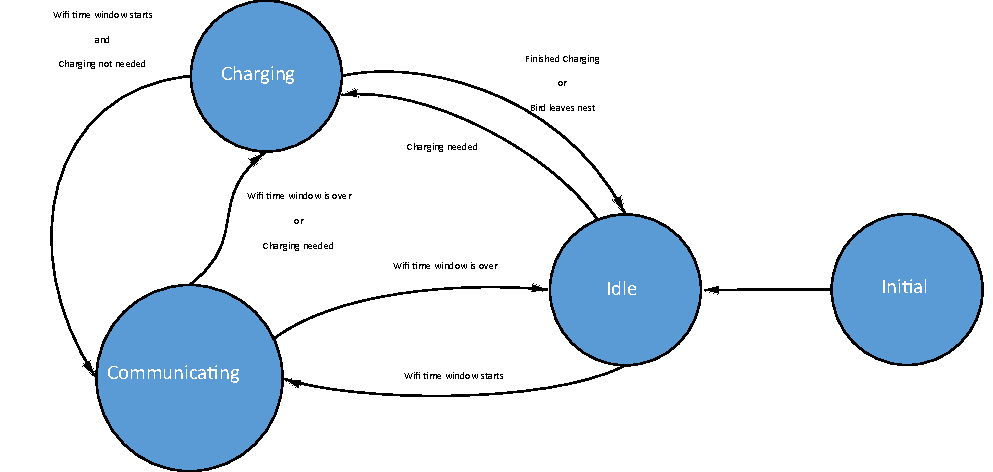
\includegraphics[width=0.9\textwidth, page=1]{ImagenesIngenieria de Detalle/FlowChart.pdf}	
	\caption{Diagrama de estados.}
	\label{fig:Diagrama_de_Estados}
\end{figure}

En el estado \textit{Initial} es aquel donde se inicializan todos los drivers, estructuras de datos y configuraciones que se encuentren por defecto. No se vuelve a este estado una vez que este haya sido abandonado. 

\begin{figure}[H]
	\centering
	%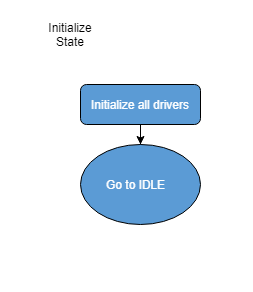
\includegraphics[width=0.4\linewidth]{ImagenesIngenieria de Detalle/diagrama_flujo_initial}	
	\includegraphics[width=0.4\textwidth, page=5]{ImagenesIngenieria de Detalle/FlowChart.pdf}	
	\caption{Diagrama de flujo: Estado Initial.}
	\label{fig:Diagrama_de_flujo_init}
\end{figure}

Luego se encuentra el estado \textit{Idle}. En este se sensan las variables físicas con el periodo de muestreo acorde a cada especificado en \lnote{PONER LUGAR DONDE ESTE ESPECIFICADO ESTO}. Luego se fija si es momento de prender el hotspot wifi. En caso afirmativo se irá al estado \textit{Communicating}. En caso contrario se analiza si hay que cargar la batería. Si se debe realizar dicha acción se irá a estado \textit{Charging}, minetras que en el caso opuesto, si hay transmisión Bluetooth, actua acorde y comienza el ciclo nuevamente.

\begin{figure}[H]
	\centering
	%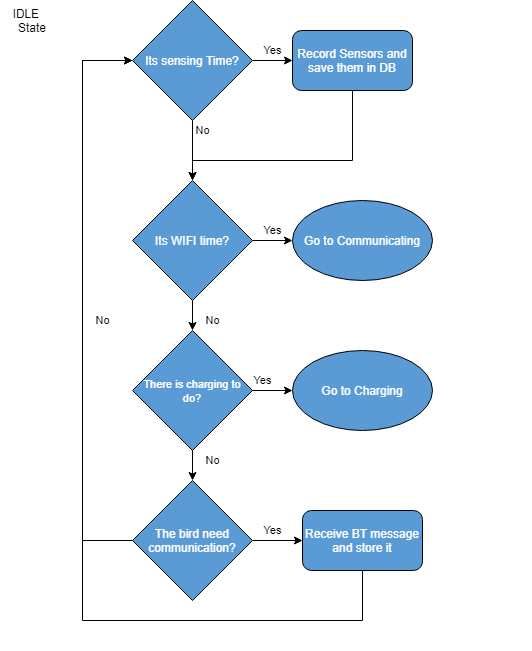
\includegraphics[width=0.9\linewidth]{ImagenesIngenieria de Detalle/diagrama_flujo_idle}	
	\includegraphics[width=0.9\textwidth, page=4]{ImagenesIngenieria de Detalle/FlowChart.pdf}	
	\caption{Diagrama de flujo: Estado \textit{Iddle}.}
	\label{fig:Diagrama_de_flujo_idle}
\end{figure}

La función principal del estado \textit{Charging} es la de cargar la UBM. Lo primero se hace en este estado es habilitar el cargador, luego, en caso de que haya un mensaje Bluetooth, se comienza la comunicación. Posteriormente se encarga del sensado, se verifica si la carga se terminó, para que cuando esto ocurra se desactive el cargador. Dependiendo si es momento de habilitar el hotspot o no se irá al estado \textit{Communicating} o \textit{Idle}.

\begin{figure}[H]
	\centering
	%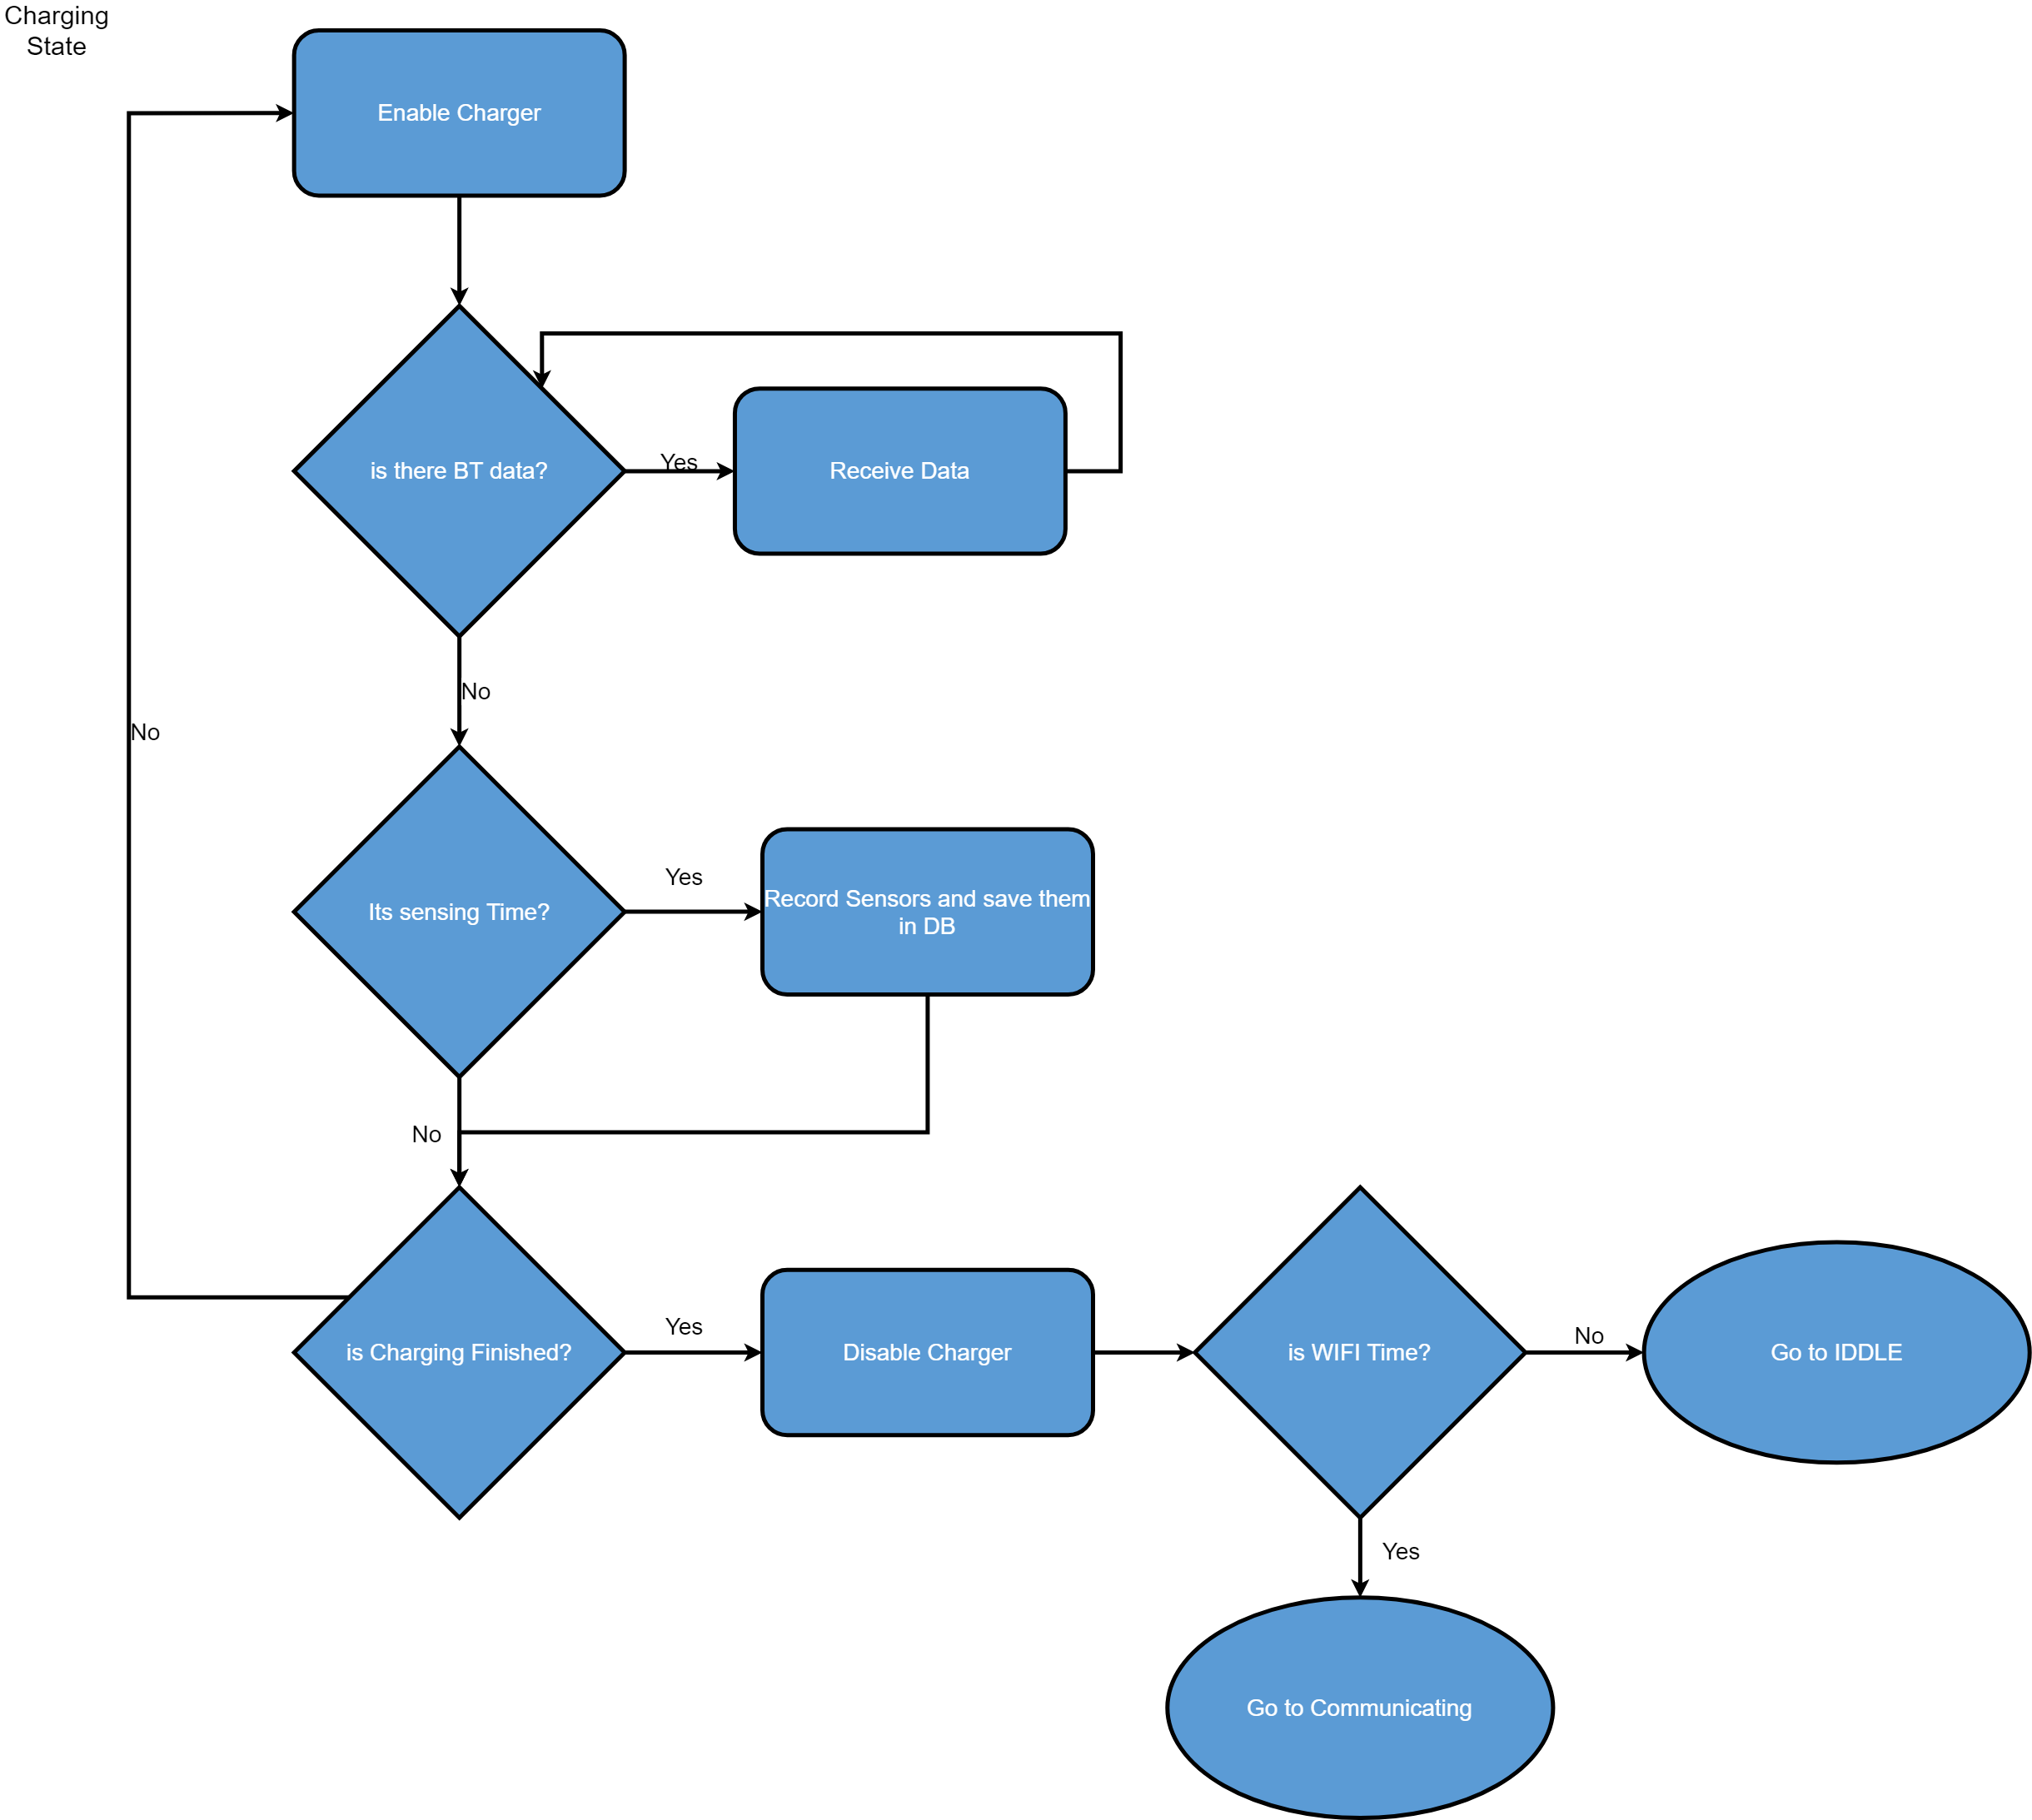
\includegraphics[width=0.9\linewidth]{ImagenesIngenieria de Detalle/diagrama_flujo_charging}	
	\includegraphics[width=0.9\textwidth, page=2]{ImagenesIngenieria de Detalle/FlowChart.pdf}
	\caption{Diagrama de flujo: Estado \textit{Charging}.}
	\label{fig:Diagrama_de_flujo_charging}
\end{figure}

Finalmente en el estado \textit{Communicating} es aquel en el que se habilita el hotspot y se levanta el servidor de Node-Red. Aquí se realiza la comunicación entre el nido y una computadora en al base del árbol. Esto se mantendrá hasta que haya pasado el tiempo especificado en \lnote{No se deberíamos decirlo en algún lado, probablemente hardware}. Además, se continua sensando las variables físicas.

\begin{figure}[H]
	\centering
	%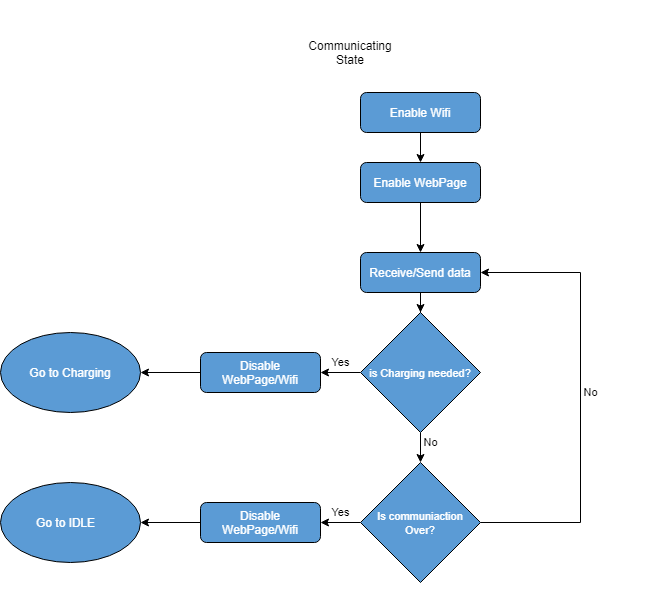
\includegraphics[width=0.9\linewidth]{ImagenesIngenieria de Detalle/diagrama_flujo_communicating}	
	\includegraphics[width=0.9\textwidth, page=3]{ImagenesIngenieria de Detalle/FlowChart.pdf}
	\caption{Diagrama de flujo: Estado \textit{Communicating}.}
	\label{fig:diagrama_flujo_communicating}
\end{figure}